% Provenance (never printed): see sources/outline_sources.md (Year 3:
% Glen's flow law; mass balance; ice sheets and ice shelves; sea ice;
% permafrost; the cryosphere's contribution to sea level).
% Brief: sources/book5/BRIEFS.md, ch. 24. Curves from figdata/bachelor-3/
% ice_flow.py (Glen slab, the plastic profile against the ETOPO1 Greenland
% transect, the Arkel ice cap) and sea_ice.py (NSIDC March and September
% extents, Stefan's law). Exercise and problem values in the Book 5 scratch
% calculator calc/ch24.py. The Arkel ice cap and the glaciers of the
% exercises are invented.
\chapter{Glaciology}\label{ch:b3:glaciology}

Cross Greenland from west to east along the parallel \ang{72.5}N. The ice
begins a few tens of kilometres inland, rises steeply, then ever more gently,
to a broad summit \qty{3229}{m} high, and falls again to the mountains of the
east coast. Plotted, the surface is close to a parabola lying on its side,
with its vertex at the margin. This chapter shows where that shape comes
from: from a material that creeps faster and faster as it is pushed harder,
so that it behaves almost as if it could not bear more than a certain stress.
It then follows the ice from the snow that feeds it to the sea that receives
it.
% ledger: data:b5-etopo-greenland

\begin{recall}
Glaciers, ice sheets, ice shelves, icebergs, sea ice, permafrost and the ice
ages are in the school books. \omterm{def:b3:deformation-mechanisms:flow-law}{Flow laws} and \omterm{def:b3:deformation-mechanisms:creep}{dislocation creep} are in
Chapter~\ref{ch:b3:deformation-mechanisms}; \omterm{def:b3:gravity-geodesy:satgrav}{satellite gravimetry} and the
ice-sheet mass balance it measures in Chapter~\ref{ch:b3:gravity-geodesy};
ice cores and their oxygen isotopes in Chapter~\ref{ch:b3:stable-isotopes}.
The sea-level budget, the ice--albedo feedback and thermosteric sea-level
rise are in the Year~2 volume, in its chapter on anthropogenic climate
change. Latent heat and heat conduction are in the physics books.
\end{recall}

\section{Ice as a material}\label{sec:b3:glaciology:material}

Glacier ice is a rock, a mass of interlocking crystals of ice, and it
deforms close to its melting point. Under a stress it creeps by the
motion of \omterm{def:b3:deformation-mechanisms:dislocation}{dislocations} in its crystals, like the rocks of
Chapter~\ref{ch:b3:deformation-mechanisms}, and its \omterm{def:b3:deformation-mechanisms:flow-law}{flow law} has the same
form: a power of the stress times an Arrhenius factor.

\begin{theorem}[Glen's flow law]\label{thm:b3:glaciology:glen}
In isotropic glacier ice the strain-rate tensor is proportional to the
deviatoric stress,
\[
\dot\varepsilon_{ij} = A(T)\,\tau_e^{\,n-1}\,\tau'_{ij}, \qquad
\tau_e^2 = \tfrac12\,\tau'_{ij}\tau'_{ij},
\]
with $n = 3$ and a \omterm{def:b3:glaciology:glen}{rate factor} $A(T)$ that grows with temperature. In
simple shear, with $\tau_{xz}$ the only non-zero deviatoric stress,
$\dot\varepsilon_{xz} = A\tau_{xz}^{\,n}$.
\end{theorem}
\index{Glen's flow law}

\begin{proof}
The law itself is empirical: a power law fitted to creep experiments and
to the deformation of glaciers, its coefficient and exponent fitted
together. In simple shear $\tau'_{xz} = \tau'_{zx} = \tau_{xz}$ and the
other components vanish, so $\tau_e^2 = \tfrac12(\tau_{xz}^2 +
\tau_{zx}^2) = \tau_{xz}^2$, and $\dot\varepsilon_{xz} = A\tau_{xz}^{\,n-1}
\tau_{xz}$.
\end{proof}
% ledger: pism:rheology

With $n = 3$, ice is a strongly non-linear fluid: doubling the stress makes
it deform eight times faster. Its effective viscosity, $1/(2A\tau_e^{\,2})$,
is not a property of the ice alone but falls as the stress rises.

\begin{definition}[Rate factor (ice)]\label{def:b3:glaciology:glen}
The \emph{rate factor}\index{rate factor (ice)} $A(T)$ of Glen's law, also
called the softness of the ice, is written $A = A_0\exp(-Q/RT)$, with an
activation energy $Q$. A widely used fit (Paterson and Budd) takes $A_0 =
\qty{3.61e-13}{s^{-1}.Pa^{-3}}$ and $Q = \qty{60}{kJ/mol}$ below
\qty{-10}{\celsius}, and $A_0 = \qty{1.73e3}{s^{-1}.Pa^{-3}}$ and $Q =
\qty{139}{kJ/mol}$ above it, closer to the melting point, where the ice
softens faster with temperature.
\end{definition}
% ledger: pism:rheology, codata:R

\begin{center}
\begin{tabular}{lccc}
\hline
temperature & \qty{-25}{\celsius} & \qty{-10}{\celsius} & \qty{0}{\celsius}\\
$A$ (\unit{Pa^{-3}.yr^{-1}}) & \num{2.7e-18} & \num{1.4e-17} & \num{1.4e-16}\\
\hline
\end{tabular}
\end{center}

Ice at its melting point flows about fifty times faster than at
\qty{-25}{\celsius} under the same stress. Stresses in glaciers are of the
order of a bar, \qty{e5}{Pa}.
% ledger: pism:rheology

A glacier moves in two ways. Its ice deforms by creep, everywhere; and
where the bed is at the melting point, it may also slide.

\begin{definition}[Basal sliding]\label{def:b3:glaciology:sliding}
\emph{Basal sliding}\index{basal sliding} is the motion of a glacier over
its bed, on a thin film of water or a layer of soft wet sediment. It
requires a bed at the melting point; a glacier frozen to its bed moves only
by the creep of its ice.
\end{definition}
% ledger: nsidc:glacier-flow

\section{Glacier flow}\label{sec:b3:glaciology:flow}

\begin{theorem}[Flow of a parallel-sided slab]\label{thm:b3:glaciology:slab}
A slab of ice of thickness $H$ and density $\rho$ lies on a bed of slope
$\alpha$ and flows down it by simple shear, sliding at speed $u_b$. At
height $z$ above the bed the shear stress is $\tau = \rho g(H - z)\sin\alpha$,
the velocity
\[
u(z) = u_b + \frac{2A}{n + 1}(\rho g\sin\alpha)^n\left[H^{n+1} - (H -
z)^{n+1}\right],
\]
and the flux per unit width $q = u_bH + \dfrac{2A}{n + 2}(\rho
g\sin\alpha)^nH^{n+2}$. The basal shear stress is $\tau_b = \rho gH\sin\alpha$.
\end{theorem}

\begin{proof}
The ice above height $z$ has weight $\rho g(H - z)$ per unit area; its
component along the slope, $\rho g(H - z)\sin\alpha$, is balanced by the
shear stress on its base, the surface being free of stress. By Glen's law,
$\mathrm du/\mathrm dz = 2\dot\varepsilon_{xz} = 2A\tau^n$; integrating from
the bed, where $u = u_b$, gives $u(z)$, and integrating $u$ from 0 to $H$
gives $q$.
\end{proof}

The velocity changes little in the upper part of the slab and fast near the
bed, where the stress is greatest: with $n = 3$ the shear is concentrated in
the lowest layers. The surface speed grows as $H^{n+1} = H^4$ and as the
cube of the slope: a glacier twice as thick flows sixteen times faster.

\begin{definition}[Shallow-ice approximation]\label{def:b3:glaciology:sia}
The \emph{shallow-ice approximation}\index{shallow-ice approximation} treats
an ice sheet whose thickness is small against its width as locally a
parallel-sided slab: at each place the ice deforms by simple shear under
the \emph{driving stress} $\tau_d = \rho gH|\nabla s|$, $s$ being the
surface elevation, and the flux follows the slab formula with the local
thickness and surface slope.
\end{definition}

In the \omterm{def:b3:glaciology:sia}{shallow-ice approximation} the basal stress is set by the shape of
the ice. Because the strain rate rises as the cube of the stress, a modest
increase of stress produces a large increase of flow, which thins the ice
and lowers the stress again: the stress stays within a narrow range,
whatever the size of the ice mass. Take this to its limit, a material that
does not deform at all below a yield stress $\tau_0$ and deforms without
limit above it, and the shape follows.

\begin{proposition}[Plastic ice-sheet profile]\label{prop:b3:glaciology:nye}
A perfectly plastic ice sheet of yield stress $\tau_0$ on a flat horizontal
bed has, at the distance $x$ inland from its margin, the surface height
\[
h(x) = \sqrt{\frac{2\tau_0x}{\rho g}} .
\]
\end{proposition}
\index{plastic ice-sheet profile}

\begin{proof}
Everywhere the basal stress equals the yield stress: $\rho gh\,\mathrm
dh/\mathrm dx = \tau_0$, the slope being small. Then $\mathrm d(h^2)/\mathrm
dx = 2\tau_0/(\rho g)$, and $h = 0$ at the margin.
\end{proof}

\begin{omfigure}
\begin{tikzpicture}
\begin{groupplot}[group style={group size=2 by 1, horizontal sep=1.5cm},
  height=0.4\linewidth,
  tick label style={font=\scriptsize}, label style={font=\small}, title style={font=\small}]
\nextgroupplot[width=0.38\linewidth, xlabel={$u/u_s$}, ylabel={height above the bed, $z/H$},
  xmin=0, xmax=1.05, ymin=0, ymax=1, title={a slab},
  legend style={font=\scriptsize, at={(0.03,0.97)}, anchor=north west}]
% computed in figdata/bachelor-3/ice_flow.py
\addplot[omThm, thick] table[x=u3, y=zeta] {figdata/out/bachelor-3-ice_flow-slab.dat};
\addlegendentry{$n = 3$}
\addplot[omDef, thick, densely dashed] table[x=u1, y=zeta] {figdata/out/bachelor-3-ice_flow-slab.dat};
\addlegendentry{$n = 1$}
\addplot[omMeth, thick] table[x=u3b, y=zeta] {figdata/out/bachelor-3-ice_flow-slab.dat};
\addlegendentry{$n = 3$, sliding}
\nextgroupplot[width=0.58\linewidth, xlabel={distance from \ang{58}W along \ang{72.5}N (\unit{km})},
  ylabel={elevation (\unit{m})}, xmin=0, xmax=1270, ymin=-500, ymax=3700,
  title={Greenland}, scaled x ticks=false, xticklabel style={/pgf/number format/1000 sep={}},
  scaled y ticks=false, yticklabel style={/pgf/number format/1000 sep={}},
  legend style={font=\scriptsize, at={(0.5,0.03)}, anchor=south}]
\addplot[black, thin] table[x=x, y=h] {figdata/out/bachelor-3-ice_flow-gl.dat};
\addlegendentry{ice and land surface}
\addplot[omThm, thick, densely dashed] table[x=x, y=h] {figdata/out/bachelor-3-ice_flow-nye-w.dat};
\addlegendentry{plastic profiles}
\addplot[omThm, thick, densely dashed, forget plot] table[x=x, y=h] {figdata/out/bachelor-3-ice_flow-nye-e.dat};
\draw[black!40] (axis cs:0,0) -- (axis cs:1270,0);
\node[font=\scriptsize, omThm, align=center] at (axis cs:330,2900) {$\tau_0 = $\\ \qty{72}{kPa}};
\node[font=\scriptsize, omThm, align=center] at (axis cs:1040,2900) {$\tau_0 = $\\ \qty{108}{kPa}};
\end{groupplot}
\end{tikzpicture}

\par\smallskip{\small Left, the velocity across a slab of ice, scaled by the
surface speed: Glen's law ($n = 3$) concentrates the shear near the bed, a
linear fluid ($n = 1$) spreads it; with sliding the whole profile is
shifted. Right, the surface of Greenland along \ang{72.5}N (ETOPO1 Ice
Surface, NOAA NCEI), and the plastic profiles fitted to its two sides, for
heights above \qty{1000}{m} and a bed taken at sea level. The fits need
yield stresses of \qty{72}{kPa} and \qty{108}{kPa}, the order of the bar of
real glaciers; they miss the steep margins, where the bed and the melting
matter.}\label{fig:b3:glaciology:flow}
\end{omfigure}
% ledger: data:b5-etopo-greenland, pism:rheology

\section{Mass balance}\label{sec:b3:glaciology:mass-balance}

A glacier is fed by snow and loses ice by melting, evaporation and, where it
reaches water, by breaking off.
% ledger: nsidc:glacier-zones

\begin{definition}[Mass balance; accumulation and ablation zones; equilibrium line]\label{def:b3:glaciology:mass-balance}
The \emph{glacier mass balance}\index{glacier mass balance} is the change
of the mass of a glacier over a year, usually given in metres of water
equivalent averaged over its area. The \emph{surface mass
balance}\index{surface mass balance} is its part due to the processes at
the surface, snowfall minus melting, runoff and sublimation; the rest is
lost by \omterm{def:b3:glaciology:grounding-line}{calving} and by melting at the base or under floating ice. The
\emph{accumulation zone}\index{accumulation zone} is the part of the
surface where the surface mass balance over a year is positive, the
\emph{ablation zone}\index{ablation zone} the part where it is negative,
and the \emph{equilibrium-line altitude}\index{equilibrium-line altitude}
(ELA) the elevation of the line between them, where it is zero.
\end{definition}

\begin{omfigure}
\centering
\begin{tikzpicture}[>=stealth, font=\small, x=1cm, y=1cm]
% bed and surface of a valley glacier, long section
\fill[black!12] (0,0) -- (0,4.6) .. controls (2,3.6) and (6,1.4) .. (11,0) -- cycle;
\fill[omSea!45] (0,4.6) .. controls (2,3.6) and (6,1.4) .. (11,0)
  -- (11,0) .. controls (8,1.0) and (4,3.2) .. (0.6,5.4) -- (0,5.6) -- cycle;
\draw[thick, black!70] (0,4.6) .. controls (2,3.6) and (6,1.4) .. (11,0);
\draw[thick, omDef] (0,5.6) -- (0.6,5.4) .. controls (4,3.2) and (8,1.0) .. (11,0);
% equilibrium line
\draw[omThm, densely dashed, thick] (5.0,2.76) -- (5.0,4.6);
\node[omThm, font=\scriptsize, anchor=south] at (5.0,4.6) {equilibrium line (ELA)};
% balance arrows
\foreach \x/\y in {1.2/5.02, 2.4/4.27, 3.6/3.56} {\draw[->, omDef, thick] (\x,\y+0.55) -- (\x,\y+0.05);}
\foreach \x/\y in {6.4/2.02, 7.6/1.42, 8.8/0.86} {\draw[->, omThm, thick] (\x,\y+0.02) -- (\x,\y+0.52);}
\node[omDef, font=\scriptsize, align=center] at (2.4,6.2) {accumulation zone:\\snow gained};
\node[omThm, font=\scriptsize, align=center] at (8.6,2.5) {ablation zone:\\ice lost};
% flow lines, computed inside the ice: buried in the accumulation zone, emerging in the ablation zone
\draw[->, black!60] plot[smooth] coordinates {(1.00,5.14) (1.98,4.28) (2.95,3.54) (3.93,2.93) (4.90,2.43) (5.88,2.00) (6.85,1.62) (7.83,1.24) (8.80,0.86)};
\draw[->, black!60] plot[smooth] coordinates {(2.20,4.39) (2.84,3.89) (3.48,3.43) (4.11,3.02) (4.75,2.67) (5.39,2.36) (6.03,2.08) (6.66,1.82) (7.30,1.56)};
\draw[->, black!60] plot[smooth] coordinates {(3.40,3.67) (3.74,3.44) (4.08,3.21) (4.41,3.00) (4.75,2.81) (5.09,2.63) (5.42,2.47) (5.76,2.32) (6.10,2.17)};
\node[font=\scriptsize, anchor=north east] at (10.9,-0.1) {snout};
\node[font=\scriptsize] at (3.0,1.4) {bedrock};
\end{tikzpicture}

\par\smallskip{\small A schematic long section of a valley glacier in
balance. Above the equilibrium line the snow of each year is buried and
carried down into the glacier; below it the surface loses ice each year and
is renewed by ice rising from depth. The flow lines (grey) dip in the
\omterm{def:b3:glaciology:mass-balance}{accumulation zone} and rise in the \omterm{def:b3:glaciology:mass-balance}{ablation zone}; the flow carries the
surplus of the one to the deficit of the other.}\label{fig:b3:glaciology:zones}
\end{omfigure}
% ledger: nsidc:glacier-zones, nsidc:glacier-flow

On the ice sheets and the high glaciers, snow is not turned into ice in a
season. It is buried by later snow, compressed, and recrystallised.

\begin{definition}[Firn; pore close-off]\label{def:b3:glaciology:firn}
\emph{Firn}\index{firn} is snow that has survived at least one melt season
and is being compacted into ice: denser than snow, still permeable to air.
\emph{Pore close-off}\index{pore close-off} is the point in its
compaction, at a density of about \qtyrange{820}{830}{kg/m^3}, where the
pores between the grains are sealed into bubbles and the air in them is cut
off from the atmosphere.
\end{definition}

On the polar ice sheets \omterm{def:b3:glaciology:firn}{pore close-off} lies \qtyrange{50}{120}{m} below the
surface, depending on the temperature, the accumulation and the
impurities; the air of an ice core's bubbles is therefore younger than the
ice around it, as Chapter~\ref{ch:b3:stable-isotopes} recalled. For most
glaciers the change from snow to ice takes more than a hundred years.
% ledger: nsidc:firn, firn:close-off

A glacier does not respond at once to a change of its climate. Its thickness
must change before its length can follow.

\begin{proposition}[Glacier response time]\label{prop:b3:glaciology:response}
A glacier of typical thickness $H$ whose balance at the terminus is $b_t <
0$ (in metres of ice per year) adjusts to a change of climate over a time of
the order of
\[
\tau = \frac{H}{-b_t} .
\]
\end{proposition}

\begin{proof}
A change of the balance by $\delta b$ over the glacier changes its volume
until the area lost or gained at the terminus, where the balance is $b_t$,
compensates it: $L\,\delta b = -b_t\,\delta L$ per unit width, for a
glacier of length $L$. The volume change needed is about $H\,\delta L$, and
the imbalance that drives it is $L\,\delta b$ per year, at first, so the
change takes $H\,\delta L/(L\,\delta b) = H/(-b_t)$ years.
\end{proof}

A glacier \qty{200}{m} thick that loses \qty{5}{m} of ice a year at its
snout needs some forty years to respond. Glaciers therefore lag the
climate: those of today will go on losing mass for decades even if the
temperature stops rising.
% ledger: ar6ch9:glaciers

\section{Ice sheets and ice shelves}\label{sec:b3:glaciology:ice-sheets}

The ice sheets of Greenland and Antarctica hold more than
\qty{99}{\percent} of the land ice. Greenland's covers \qty{1.7}{\mega
km^2} and is more than \qty{3}{km} thick at most; Antarctica's covers
almost \qty{14}{\mega km^2} and is nearly \qty{4.9}{km} thick at most. Many
parts of the Antarctic ice sheet rest on a bed below sea level.
% ledger: nsidc:ice-sheets, ar6ch9:faq91

\begin{definition}[Ice stream]\label{def:b3:glaciology:ice-stream}
An \emph{ice stream}\index{ice stream} is a band of an ice sheet that flows
much faster than the ice on either side of it, mostly by sliding or by the
deformation of a soft wet bed, and drains a large part of the ice sheet's
interior towards its margin.
\end{definition}

\begin{definition}[Grounding line; calving]\label{def:b3:glaciology:grounding-line}
The \emph{grounding line}\index{grounding line} is the line where ice
resting on its bed begins to float: seaward of it the ice is an ice shelf
or a floating glacier tongue. \emph{Calving}\index{calving} is the breaking
off of blocks of ice, icebergs, at the front of a glacier or an ice shelf
that ends in water.
\end{definition}

Ice shelves float, so their melting does not raise sea level. But they are
held at their sides and on the rises of the sea floor where they run
aground, and the drag there resists the flow of the ice behind: they
\emph{buttress} it. After the Larsen~B ice shelf disintegrated in 2002, the
glaciers that had fed it sped up, up to eight times.
% ledger: nsidc:ice-shelves

\begin{proposition}[Flotation]\label{prop:b3:glaciology:flotation}
Ice of density $\rho_i$ and thickness $H$ over a bed at depth $D$ below sea
level, in sea water of density $\rho_w$, floats if $H < (\rho_w/\rho_i)D$.
With $\rho_i = \qty{917}{kg/m^3}$ and $\rho_w = \qty{1025}{kg/m^3}$, the
\omterm{def:b3:glaciology:grounding-line}{grounding line} lies where the ice is $1.12\,D$ thick.
\end{proposition}

\begin{proof}
Floating ice displaces its own weight of water: a column of thickness $H$
needs a draught $\rho_iH/\rho_w$. If the water is deeper than that draught,
the ice floats.
\end{proof}
% ledger: iapws:ice-density, noaa:seawater-1025

\begin{omfigure}
\centering
\begin{tikzpicture}[>=stealth, font=\small, x=1cm, y=1cm]
% sea and bed
\fill[omSea!50] (4.2,0) rectangle (11,-2.8);
\fill[black!15] (0,-0.9) -- (2.2,-2.0) -- (4.6,-1.6) -- (7.0,-2.3) -- (11,-2.6)
  -- (11,-3.2) -- (0,-3.2) -- cycle;
\draw[thick, black!60] (0,-0.9) -- (2.2,-2.0) -- (4.6,-1.6) -- (7.0,-2.3) -- (11,-2.6);
% grounded ice and ice shelf
\fill[white] (0,-0.9) -- (0,2.4) .. controls (2,2.2) and (3.6,1.4) .. (4.6,0.2)
  -- (9.2,0.12) -- (9.2,-1.0) -- (4.6,-1.6) -- (2.2,-2.0) -- cycle;
\draw[thick, omDef] (0,2.4) .. controls (2,2.2) and (3.6,1.4) .. (4.6,0.2) -- (9.2,0.12)
  -- (9.2,-1.0) -- (4.6,-1.6);
\draw[thick] (0,0) -- (0,0);
\draw[omDef!60, thin] (0,0) -- (4.3,0); \draw[omDef!60, thin] (9.2,0) -- (11,0);
\node[font=\scriptsize, anchor=south west] at (0.05,0.02) {sea level};
% icebergs
\fill[white] (10.1,0.1) rectangle (10.6,-0.7); \draw[omDef] (10.1,0.1) rectangle (10.6,-0.7);
% labels
\fill[omThm] (4.6,-1.6) circle (0.07);
\draw[omThm, ->] (4.0,-2.6) node[anchor=north, font=\scriptsize] {grounding line} -- (4.55,-1.68);
\node[font=\scriptsize] at (1.4,1.1) {grounded ice sheet};
\node[font=\scriptsize] at (6.9,-0.7) {floating ice shelf};
\node[font=\scriptsize, anchor=south] at (9.2,0.2) {calving front};
\node[font=\scriptsize, anchor=north, align=center] at (10.35,-0.8) {iceberg};
\node[font=\scriptsize, align=center] at (2.1,-2.55) {bed deepening\\inland};
\draw[->, black!60, thick] (2.2,1.6) -- (3.6,1.0);
\draw[->, black!60, thick] (5.4,-0.2) -- (7.0,-0.2);
\node[font=\scriptsize, align=center, omMeth] at (7.0,1.2) {buttressing: drag at the shelf's\\sides and grounded rises};
\draw[->, omMeth, thick] (7.6,0.6) -- (6.6,0.6);
\end{tikzpicture}

\par\smallskip{\small A schematic section of a marine ice sheet, not to
scale. The ice rests on a bed below sea level, which deepens inland; at the
\omterm{def:b3:glaciology:grounding-line}{grounding line} it begins to float, as an ice shelf, which loses ice by
\omterm{def:b3:glaciology:grounding-line}{calving} at its front and by melting from below. The drag on the shelf where
it is held at its sides and on rises of the sea floor resists the flow of
the grounded ice.}\label{fig:b3:glaciology:grounding}
\end{omfigure}
% ledger: nsidc:ice-shelves, ar6ch9:misi

On a bed that deepens inland the \omterm{def:b3:glaciology:grounding-line}{grounding line} is fragile. Where the
water is deeper, the ice at the \omterm{def:b3:glaciology:grounding-line}{grounding line} is thicker, by the flotation
condition, and by the slab theorem the flux of a thicker column grows
steeply with its thickness. If the \omterm{def:b3:glaciology:grounding-line}{grounding line} retreats down such a
slope, it reaches thicker ice that discharges more, thins faster, and lets
the line retreat further.

\begin{definition}[Marine ice-sheet instability]\label{def:b3:glaciology:misi}
\emph{Marine ice-sheet instability}\index{marine ice-sheet instability}
(MISI) is the proposed self-reinforcing retreat of the \omterm{def:b3:glaciology:grounding-line}{grounding line} of an
ice sheet resting on a bed that slopes down towards the interior: without
the buttressing of an ice shelf, the \omterm{def:b3:glaciology:grounding-line}{grounding line} on such a bed is
inherently unstable until it reaches a bed sloping upward.
\end{definition}

Ice shelves can hold a \omterm{def:b3:glaciology:grounding-line}{grounding line} in place even on a downward slope.
Models in which all the Antarctic ice shelves are removed and not allowed
to reform lose ice equivalent to \qtyrange{2}{10}{m} of sea level in 500
years through this instability, \qtyrange{2}{5}{m} of it from West
Antarctica. On ice sheets resting mostly on bedrock above sea level, like
Greenland, the main self-reinforcing process is another: as the surface
melts and lowers, it lies in warmer air and melts more.
% ledger: ar6ch9:misi, ar6ch9:faq91

\begin{definition}[Sea-level equivalent]\label{def:b3:glaciology:sle}
The \emph{sea-level equivalent}\index{sea-level equivalent} of a mass of
land ice is the rise of the global mean sea level that its melting would
cause if the water spread over the present ocean.
\end{definition}

\begin{proposition}[Sea-level equivalent of a mass of ice]\label{prop:b3:glaciology:sle}
A mass $M$ of ice resting above sea level, spread over an ocean of area
$A_o$ as water of density $\rho_w$, raises the sea level by $M/(\rho_wA_o)$:
about \qty{1}{mm} for each \qty{360}{Gt}.
\end{proposition}

\begin{proof}
The water occupies the volume $M/\rho_w$ over the area $A_o$. With the
\qty{360}{Gt} per millimetre adopted by the ice-sheet mass-balance
assessments, $A_o\rho_w = \qty{3.6e17}{kg/m}$: an ocean of about
\qty{3.6e8}{km^2} for water of the density of fresh water.
\end{proof}
% ledger: data:b5-imbie

Ice already below sea level displaces sea water, so it counts for less:
Antarctica's \qty{30}{\mega km^3} of ice are equivalent to about
\qty{58}{m} of sea level, less than its mass divided by
\qty{360}{Gt/mm}.
% ledger: nsidc:ice-sheets

\begin{omfigure}
\centering
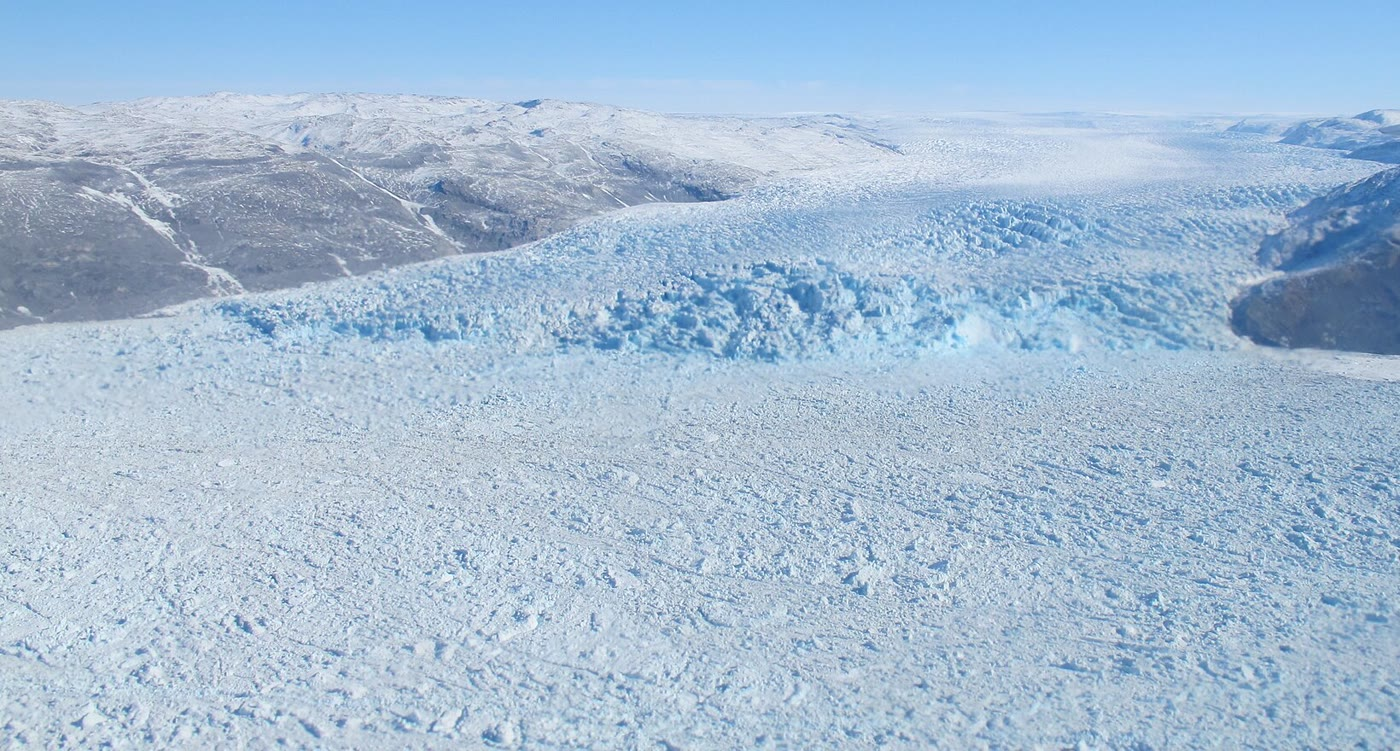
\includegraphics[width=0.82\linewidth]{images/book5/b3-greenland-outlet.jpg}

\par\smallskip{\small An outlet glacier of the Greenland ice sheet,
between mountains, ending in the sea at its \omterm{def:b3:glaciology:grounding-line}{calving} front, the broken wall
of blue ice across the middle of the picture; the fjord in front is choked
with calved ice and sea ice. Photographed from an aircraft of NASA's
Operation IceBridge in April 2014 (NASA / Jim Yungel, public
domain).}\label{fig:b3:glaciology:outlet}
\end{omfigure}
% ledger: photo:b3-greenland-outlet

\begin{inthefield}[A camp on the ice]
\begin{minipage}[t]{0.55\linewidth}\vspace{0pt}
On an ice sheet the glaciologists' instruments travel by sledge and live in
tents. To measure how fast the ice moves, they freeze a pole into the
snow and mount on it the antenna of a satellite-navigation receiver. The
receivers used in geodesy fix a position to within a few centimetres, so
positions repeated over weeks or seasons give the speed and the direction
of the ice, and the height of the pole, surveyed again, the thinning or
thickening of the ice beneath it.
\end{minipage}\hfill
\begin{minipage}[t]{0.42\linewidth}\vspace{0pt}
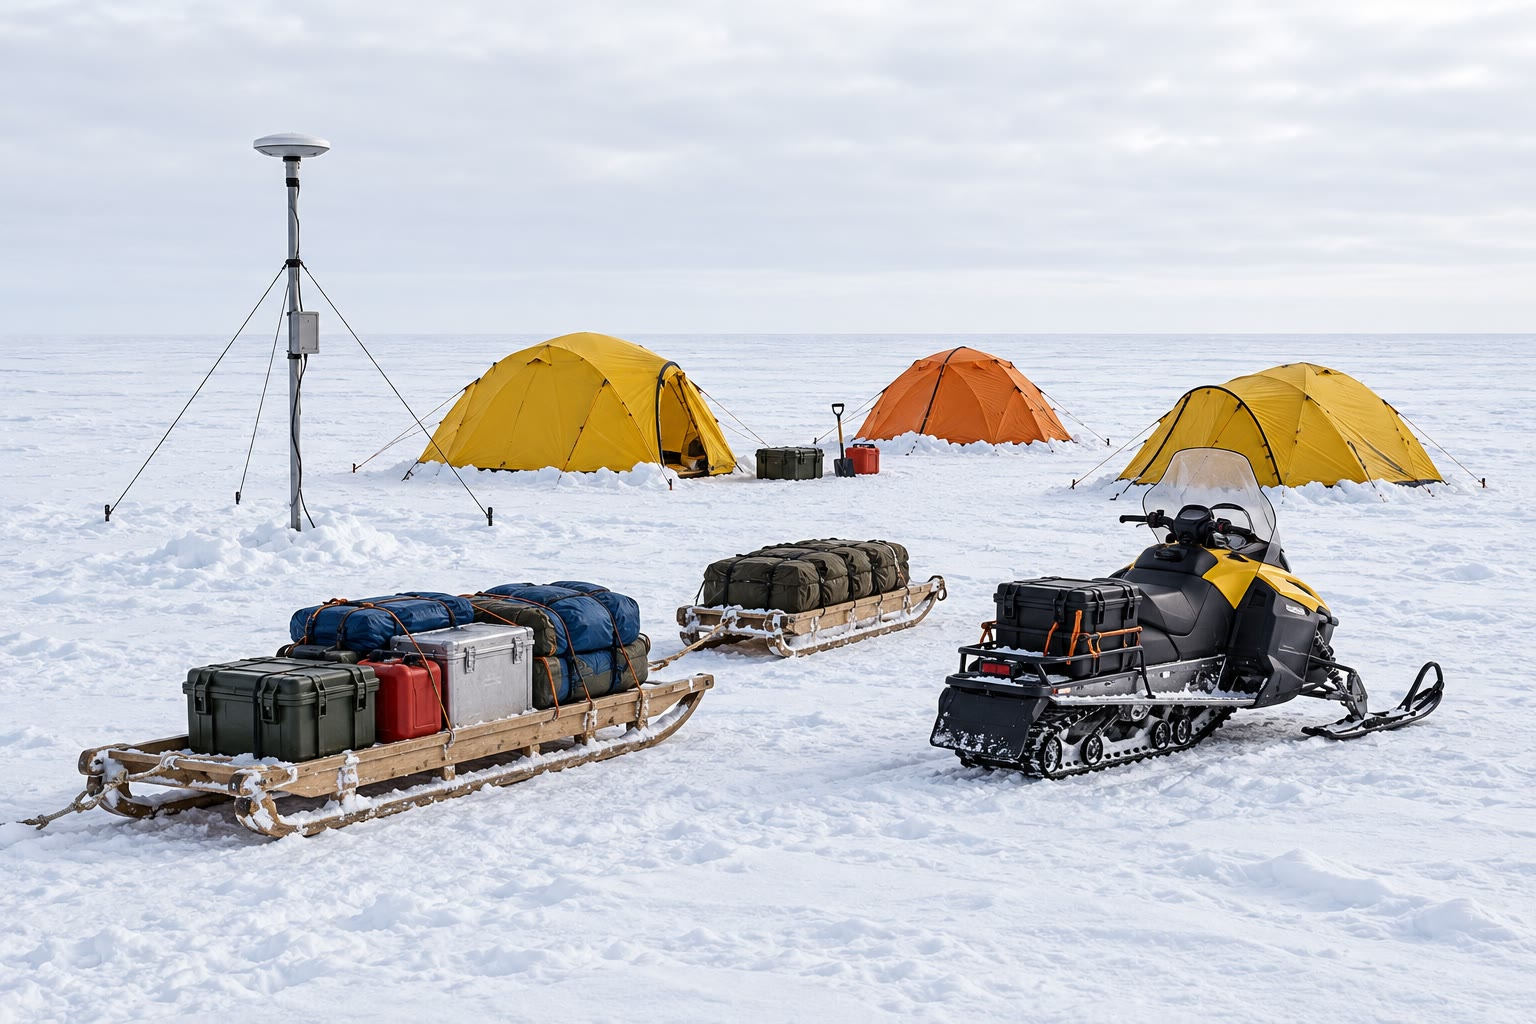
\includegraphics[width=\linewidth]{images/book5/ai/b3-glaciology-camp.jpg}

{\scriptsize A field camp on an ice sheet: tents, sledges and a
snowmobile, and a satellite-navigation antenna on a mast held by guy
lines (AI-generated illustration).}
\end{minipage}
\end{inthefield}
% ledger: gps:high-end

\section{Sea ice and permafrost}\label{sec:b3:glaciology:sea-ice}

Sea ice forms, grows and melts in the ocean. In the Arctic it reaches its
largest area in March and its smallest in September.
% ledger: nsidc:sea-ice-def

\begin{definition}[Sea-ice extent]\label{def:b3:glaciology:sea-ice}
The \emph{sea-ice extent}\index{sea-ice extent} is the total area of the
cells of a satellite map in which sea ice covers more than
\qty{15}{\percent} of the surface. It is larger than the sea-ice area,
which counts only the ice itself.
\end{definition}
% ledger: nsidc:sea-ice-def

Since satellites began to map it in 1979 the Arctic extent has shrunk, in
March and much more in September: by \qty{0.74}{\mega km^2} per decade in
September, about \qty{12}{\percent} of the 1981--2010 mean per decade, against
\qty{0.38}{\mega km^2}, \qty{2.5}{\percent}, in March. The smallest
September extent so far, \qty{3.57}{\mega km^2}, was in 2012. Arctic sea
ice reflects \qtyrange{50}{70}{\percent} of the sunlight, the open ocean
about \qty{6}{\percent}: losing the ice darkens the surface, the ice--albedo
feedback of the Year~2 volume.
% ledger: data:b5-nsidc-extent, nsidc:sea-ice-reflect

Sea ice grows at its base, where sea water freezes on it, and the latent
heat of that freezing must be conducted up through the ice to the cold air.

\begin{theorem}[Stefan's law]\label{thm:b3:glaciology:stefan}
Sea ice of thermal conductivity $k_i$, density $\rho_i$ and latent heat of
fusion $L$, its surface held at a temperature $\Delta T$ below the freezing
point of the water beneath, grows, if the heat from the ocean is
negligible, as
\[
h(t)^2 - h(0)^2 = \frac{2k_i\,\Delta T}{\rho_iL}\,t .
\]
Under a layer of snow of thickness $h_s$ and conductivity $k_s$ the growth
rate is $\mathrm dh/\mathrm dt = \Delta T/[\rho_iL(h/k_i + h_s/k_s)]$.
\end{theorem}

\begin{proof}
The temperature in the thin ice is linear, from the freezing point at the
base to the surface temperature at the top, so the heat flux through it is
$k_i\Delta T/h$, or, through ice and snow in series, $\Delta T/(h/k_i +
h_s/k_s)$. Freezing a layer $\mathrm dh$ releases $\rho_iL\,\mathrm dh$ per
unit area, which this flux must carry away: $\rho_iL\,\mathrm dh/\mathrm dt
= k_i\Delta T/h$. Then $\mathrm d(h^2)/\mathrm dt = 2k_i\Delta T/(\rho_iL)$.
\end{proof}

With $k_i = \qty{2.03}{W.m^{-1}.K^{-1}}$, $L = \qty{3.34e5}{J/kg}$ and
$\rho_i = \qty{917}{kg/m^3}$, a surface \qty{20}{K} below freezing grows
\qty{1.5}{m} of ice in a hundred days and \qty{2.1}{m} in two hundred.
Snow, with a conductivity of \qty{0.30}{W.m^{-1}.K^{-1}}, is a good
insulator: \qty{20}{cm} of it more than halves the growth. Thick ice grows
slowly, thin ice fast: the law tends to even out the thickness of the ice
after a summer of melting.
% ledger: cice:constants, iapws:ice-density

\begin{omfigure}
\begin{tikzpicture}
\begin{groupplot}[group style={group size=2 by 1, horizontal sep=1.5cm},
  width=0.48\linewidth, height=0.4\linewidth,
  tick label style={font=\scriptsize}, label style={font=\small}, title style={font=\small}]
\nextgroupplot[xlabel={year}, ylabel={extent (\unit{\mega km^2})}, xmin=1977, xmax=2028,
  ymin=0, ymax=18, title={Arctic sea-ice extent},
  xticklabel style={/pgf/number format/1000 sep={}},
  legend style={font=\scriptsize, at={(0.03,0.66)}, anchor=west}]
% computed in figdata/bachelor-3/sea_ice.py
\addplot[omDef, thick, mark=*, mark size=0.9pt] table[x=year, y=mar] {figdata/out/bachelor-3-sea_ice-extent.dat};
\addlegendentry{March}
\addplot[omThm, thick, mark=*, mark size=0.9pt] table[x=year, y=sep] {figdata/out/bachelor-3-sea_ice-extent.dat};
\addlegendentry{September}
\addplot[black!60, densely dashed, forget plot] table[x=year, y=mar] {figdata/out/bachelor-3-sea_ice-trend.dat};
\addplot[black!60, densely dashed, forget plot] table[x=year, y=sep] {figdata/out/bachelor-3-sea_ice-trend.dat};
\nextgroupplot[xlabel={days of freezing}, ylabel={ice thickness (\unit{m})}, xmin=0, xmax=200,
  ymin=0, ymax=2.4, title={growth, $\Delta T = \qty{20}{K}$},
  legend style={font=\scriptsize, at={(0.97,0.03)}, anchor=south east}]
\addplot[omMeth, thick] table[x=day, y=h0] {figdata/out/bachelor-3-sea_ice-stefan.dat};
\addlegendentry{bare ice}
\addplot[omDef, thick, densely dashed] table[x=day, y=hs] {figdata/out/bachelor-3-sea_ice-stefan.dat};
\addlegendentry{under \qty{20}{cm} of snow}
\end{groupplot}
\end{tikzpicture}

\par\smallskip{\small Left, the mean Arctic \omterm{def:b3:glaciology:sea-ice}{sea-ice extent} in March and in
September, 1979--2026 (NSIDC Sea Ice Index, version~4), with least-squares
trends (dashed): \qty{-0.38}{\mega km^2} and \qty{-0.74}{\mega km^2} per
decade. Right, the growth of sea ice by conduction under a surface
\qty{20}{K} below freezing, without ocean heat: bare ice by Stefan's law,
and the same ice under \qty{20}{cm} of snow.}\label{fig:b3:glaciology:sea-ice}
\end{omfigure}
% ledger: data:b5-nsidc-extent, cice:constants

Permafrost is ground that stays at or below \qty{0}{\celsius} for two years
or more. It underlies about a quarter of the exposed land of the Northern
Hemisphere.
% ledger: nsidc:permafrost

\begin{definition}[Active layer]\label{def:b3:glaciology:permafrost}
The \emph{active layer}\index{active layer} is the layer of ground above
the permafrost that thaws each summer and freezes again each winter.
\end{definition}

Its thickness is set, like the growth of sea ice, by the conduction of heat
into the ground during the thaw season, against the latent heat of the
ground's ice. Permafrost temperatures have increased over the past three to
four decades throughout the permafrost regions (high confidence);
permafrost warmed globally by \qty{0.29}{\celsius} [\numrange{0.17}{0.41}]
between 2007 and 2016 (medium confidence), and an increase of the
active-layer thickness is a pan-Arctic phenomenon (medium confidence).
Where its ice melts, the ground can collapse.
% ledger: ar6ch9:permafrost, nsidc:permafrost-thaw

\section{The cryosphere and sea level}\label{sec:b3:glaciology:sea-level}

The sea-level budget of the Year~2 volume adds the expansion of the warming
ocean to the water added by the ice and by the land. Of the
\qty{3.69}{mm/yr} of sea-level rise observed over 2006--2018, glaciers
contributed \qty{0.62}{mm/yr}, Greenland \qty{0.63}{mm/yr} and Antarctica
\qty{0.37}{mm/yr}: the ice together more than the expansion of the ocean,
\qty{1.39}{mm/yr}.
% ledger: ar6ch9:table95

\begin{dated}{2021}
Greenland lost \qty{4890}{Gt} of ice over 1992--2020 [4140 to 5640],
\qty{13.5}{mm} of sea level, at rates rising from \qty{39}{Gt/yr} in the
1990s to \qty{243}{Gt/yr} in 2010--2019, by discharge and, increasingly,
by surface melt (high confidence). Antarctica lost \qty{2670}{Gt}
[1800 to 3540], \qty{7.4}{mm}, its rate rising from \qty{49}{Gt/yr} in the
1990s to \qty{148}{Gt/yr} in 2010--2019; the losses came from the outlet glaciers of West
Antarctica, mainly through the melting of the ice shelves from below (high
confidence). The glaciers outside the ice sheets lost \qty{6200}{Gt} over
1993--2019, \qty{17.1}{mm}, more in 2010--2019 than in any other decade of
the record (very high confidence). Greenland will continue to lose mass
throughout this century under all the scenarios considered (virtually
certain), and so will Antarctica (likely): by 2100 Greenland likely adds
\qtyrange{0.01}{0.10}{m} to the sea level under a low-emissions scenario
and \qtyrange{0.09}{0.18}{m} under a very high one, Antarctica
\qtyrange{0.03}{0.27}{m} and \qtyrange{0.03}{0.34}{m}. The Arctic Ocean
will likely become practically free of sea ice, with less than
\qty{1}{\mega km^2} of it, at its September minimum for the first time
before 2050 under all the scenarios considered.
\end{dated}
% ledger: ar6ch9:greenland, ar6ch9:antarctica, ar6ch9:glaciers, ar6ch9:ice-sheet-proj, ar6ch9:sea-ice

The ice-sheet losses are those of Chapter~\ref{ch:b3:gravity-geodesy},
measured by altimetry, by gravimetry and by the difference between the snow
that falls and the ice that flows out: three independent methods brought
into one estimate.
% ledger: data:b5-imbie

\section{Exercises}

\begin{exercise}[$\star$]\label{exo:b3:glaciology:1}
A valley glacier \qty{250}{m} thick flows down a slope of \ang{3}. Compute
the basal shear stress, and compare it with the basal stresses of real
glaciers, of the order of a bar.
\end{exercise}

\begin{exercise}[$\star$]\label{exo:b3:glaciology:2}
(a)~The Greenland ice sheet holds about \qty{2.9}{\mega km^3} of ice of
density \qty{917}{kg/m^3}. Compute its mass and its \omterm{def:b3:glaciology:sle}{sea-level equivalent} at
\qty{360}{Gt/mm}, and compare with the \qty{7.4}{m} usually quoted.
(b)~Do the same for Antarctica's \qty{30}{\mega km^3}, quoted as about
\qty{58}{m}. Why do the two compare so differently?
\end{exercise}
% ledger: nsidc:ice-sheets

\begin{exercise}[$\star$]\label{exo:b3:glaciology:3}
A glacier has an \omterm{def:b3:glaciology:mass-balance}{accumulation zone} of \qty{6}{km^2} with a mean balance of
\qty{+1.2}{m} water equivalent, and an \omterm{def:b3:glaciology:mass-balance}{ablation zone} of \qty{4}{km^2} with
\qty{-2.1}{m}. Compute its net balance in cubic metres of water, its mean
specific balance, and its accumulation-area ratio. Is it growing or
shrinking?
\end{exercise}

\begin{exercise}[$\star$]\label{exo:b3:glaciology:4}
At \omterm{def:b3:glaciology:firn}{pore close-off} the \omterm{def:b3:glaciology:firn}{firn} has a density of \qtyrange{820}{830}{kg/m^3}.
What fraction of its volume is still pore space (ice:
\qty{917}{kg/m^3})?
\end{exercise}
% ledger: firn:close-off

\begin{exercise}[$\star\star$]\label{exo:b3:glaciology:5}
A temperate glacier (ice at \qty{0}{\celsius}, $A =
\qty{1.4e-16}{Pa^{-3}.yr^{-1}}$) is \qty{300}{m} thick on a slope of
\ang{3}. Compute its surface speed by internal deformation alone. By what
factor would the speed change if it were twice as thick? If the slope were
halved?
\end{exercise}

\begin{exercise}[$\star\star$]\label{exo:b3:glaciology:6}
From the Paterson--Budd constants, compute the \omterm{def:b3:glaciology:glen}{rate factor} at
\qty{-25}{\celsius} and \qty{-10}{\celsius}, and the ratio of the speeds of
two identical ice masses at \qty{0}{\celsius} and at \qty{-25}{\celsius}.
\end{exercise}
% ledger: pism:rheology, codata:R

\begin{exercise}[$\star\star$]\label{exo:b3:glaciology:7}
Compute the greatest thickness of a plastic ice sheet \qty{1000}{km} from
centre to margin with $\tau_0 = \qty{100}{kPa}$, and compare with the
greatest thickness of the Antarctic ice, nearly \qty{4.9}{km}.
\end{exercise}
% ledger: nsidc:ice-sheets

\begin{exercise}[$\star\star$]\label{exo:b3:glaciology:8}
A glacier \qty{200}{m} thick loses \qty{5}{m} of ice a year at its snout.
Estimate its response time. If the climate warmed abruptly and then stayed
constant, how long would its length go on changing?
\end{exercise}

\begin{exercise}[$\star\star$]\label{exo:b3:glaciology:9}
(a)~Using Stefan's law with $\Delta T = \qty{20}{K}$, compute the thickness
of bare sea ice after 100 days, and the time needed to reach \qty{3}{m}.
(b)~What does this suggest about ice thicker than \qty{3}{m}?
\end{exercise}
% ledger: cice:constants

\begin{exercise}[$\star\star\star$]\label{exo:b3:glaciology:10}
(a)~Where the bed is \qty{800}{m} below sea level, how thick is the ice at
the \omterm{def:b3:glaciology:grounding-line}{grounding line}? (b)~Using the slab flux $q \propto H^{n+2}$ for a given
surface slope, by what factor does the flux of the grounded ice rise if the
\omterm{def:b3:glaciology:grounding-line}{grounding line} retreats to where the bed is \qty{900}{m} deep? (c)~Explain
why a bed deepening inland makes the retreat self-reinforcing, and what an
ice shelf changes.
\end{exercise}
% ledger: iapws:ice-density, noaa:seawater-1025

\begin{exercise}[$\star\star\star$]\label{exo:b3:glaciology:11}
Show that the volume of a circular plastic ice cap of radius $R$ is $V =
\frac{8\pi}{15}\sqrt{2\tau_0/(\rho g)}\,R^{5/2}$. By what factor does its
\omterm{def:b3:glaciology:sle}{sea-level equivalent} grow if its radius doubles?
\end{exercise}

\begin{exercise}[$\star\star\star$]\label{exo:b3:glaciology:12}
The mean Arctic extent was \qty{16.34}{\mega km^2} in March 1979 and
\qty{14.13}{\mega km^2} in March 2026; in September, \num{7.05} and
\qty{4.81}{\mega km^2}. (a)~Compute the relative change in each month.
(b)~Give two physical reasons why the September extent has fallen so much
faster than the March extent.
\end{exercise}
% ledger: data:b5-nsidc-extent

\section{Problem: The Arkel Ice Cap}

\begin{problem}[{Weekend problem --- the shape, flow, balance and
sea-level equivalent of an invented ice cap}]
\label{pb:b3:glaciology:1}
The invented Arkel ice cap lies on a flat plateau. It is nearly circular,
\qty{20}{km} in radius, and its ice is at about \qty{-10}{\celsius}. Take
$\rho = \qty{917}{kg/m^3}$ and $g = \qty{9.81}{m/s^2}$.

\medskip\noindent\textbf{Part I --- Is the cap plastic?}
\begin{enumerate}
\item Show that under ice of thickness $H$ with a small surface slope
  $\alpha$ the basal shear stress is about $\rho gH\alpha$.
\item Radar soundings and surveys at 5, 10 and \qty{15}{km} from the centre
  give thicknesses of 580, 470 and \qty{335}{m} and surface slopes of
  \num{0.0190}, \num{0.0240} and \num{0.0330}. Compute the basal shear
  stress at the three points.
\item Is the cap close to plastic? What yield stress do you adopt?
\item With $\tau_0 = \qty{100}{kPa}$, compute $2\tau_0/(\rho g)$.
\item Predict the thickness at the three points from the plastic profile
  and compare with the soundings.
\end{enumerate}

\medskip\noindent\textbf{Part II --- Shape and volume.}
\begin{enumerate}[resume]
\item Compute the thickness at the centre.
\item Show that the volume is $V = \frac{8\pi}{15}\sqrt{2\tau_0/(\rho
  g)}\,R^{5/2}$.
\item Compute the volume in cubic kilometres.
\item Compute the area and the mean thickness.
\item An ice cap twice as wide on the same plateau: by what factor is its
  volume larger?
\end{enumerate}

\medskip\noindent\textbf{Part III --- Flow and balance.}
\begin{enumerate}[resume]
\item Compute the \omterm{def:b3:glaciology:glen}{rate factor} at \qty{-10}{\celsius} in
  \unit{Pa^{-3}.yr^{-1}}.
\item At \qty{10}{km} from the centre, treating the ice as a slab, compute
  the surface speed by internal deformation.
\item Compute the ice flux per unit width there, and the mean velocity of
  the column.
\item In a steady state, the flux leaving the circle of radius
  \qty{10}{km} equals the balance gained inside it. What mean balance, in
  metres of ice per year, does this require?
\item The equilibrium line lies \qty{450}{m} above the plateau. Where is it
  on the cap, and what is the accumulation-area ratio?
\item If the ice warmed to \qty{0}{\celsius}, by what factor would the
  speeds rise? What would happen to the cap's shape?
\end{enumerate}

\medskip\noindent\textbf{Part IV --- Sea level.}
\begin{enumerate}[resume]
\item Compute the mass of the cap in gigatonnes.
\item Compute its \omterm{def:b3:glaciology:sle}{sea-level equivalent} in millimetres.
\item If the whole cap thinned by \qty{0.5}{m} of ice a year, without
  flowing, how long would it last?
\item Why would the real cap disappear sooner than that, once it began to
  thin?
\item At the rate at which Greenland lost ice in 2010--2019, how long would
  it take to lose a mass equal to the Arkel cap?
\item Give the \omterm{def:b3:glaciology:sle}{sea-level equivalent} of the Arkel ice cap, in millimetres,
  to one decimal.
\end{enumerate}
\end{problem}
% ledger: pism:rheology, data:b5-imbie, ar6ch9:greenland, ar6ch9:faq91
